%File: paper_v0.tex
\documentclass[letterpaper]{article} % DO NOT CHANGE THIS
\usepackage[submission]{aaai2026}  % DO NOT CHANGE THIS
\usepackage{times}  % DO NOT CHANGE THIS
\usepackage{helvet}  % DO NOT CHANGE THIS
\usepackage{courier}  % DO NOT CHANGE THIS
\usepackage[hyphens]{url}  % DO NOT CHANGE THIS
\usepackage{graphicx} % DO NOT CHANGE THIS
\urlstyle{rm} % DO NOT CHANGE THIS
\def\UrlFont{\rm}  % DO NOT CHANGE THIS
\usepackage{natbib}  % DO NOT CHANGE THIS AND DO NOT ADD ANY OPTIONS TO IT
\usepackage{caption} % DO NOT CHANGE THIS AND DO NOT ADD ANY OPTIONS TO IT
\frenchspacing  % DO NOT CHANGE THIS
\setlength{\pdfpagewidth}{8.5in} % DO NOT CHANGE THIS
\setlength{\pdfpageheight}{11in} % DO NOT CHANGE THIS

% Additional packages (not on the AAAI disallowed list)
\usepackage{booktabs}
\usepackage{array}
\usepackage{amsmath}
\usepackage{amssymb}
\usepackage{enumitem}

\pdfinfo{
/TemplateVersion (2026.1)
}

\setcounter{secnumdepth}{0}

\title{It's the Humans, Not the Data:\\
Geopolitical Bias in {LLM}s Is a Post-Training Decision,\\
Amplified by the Language of the Prompt}

\author{
    Anonymous Submission
}
\affiliations{
    %
}

\begin{document}

\maketitle

\begin{abstract}
\noindent Geopolitical bias in open-weight LLMs is installed by post-training, not by the pretraining corpus, and the language of the prompt at inference time decides how much of it surfaces. We test this on fourteen models---seven families from seven labs, each with matched base and post-trained variants---using a paired-scenario forced-choice probe across 28 country pairs in English, French, and Chinese. Base models across all seven families rate countries near-equally (cross-country spread $\sigma \leq 9.3$ log-odds on China-favourability); their post-trained variants do not ($\sigma$ up to $22$). The sharpest test is Qwen~2.5: its base, pretrained primarily on Chinese-language corpora, sits at $-0.19$ on China-favourability (near neutral); the chat variant Alibaba shipped on top is at $+2.99$. A ``Chinese data $\to$ pro-China output'' story predicts a pattern we do not observe. The direction of the post-training shift also tracks the maker's nationality for 6 of 7 families (01.AI's Yi is a counter-example, visible only after a response-template correction); magnitudes are heterogeneous---only Alibaba's Qwen ends in clearly pro-China absolute territory. At inference time, prompting the post-trained models in Chinese pushes 5/7 further pro-China, and prompting the French-made Mistral in French is the unique combination that produces a positive France-favourability in our sample (EN $-1.60 \to$ FR $+0.37$). Base models barely respond to either language switch. The bias-installation step is the post-training pipeline; the language switch is the dial that turns it up.
\end{abstract}

\section{Introduction}

When a language model is asked to adjudicate a geopolitical event---whose military action was justified, which government's response was measured---whose side does it take? And \emph{when} does it take a side?

We make one primary claim, sharper than the obvious ``pretraining data is biased, so the model is biased.''

\paragraph{Post-training, not pretraining, creates geopolitical preferences in open-weight LLMs.} Base models across seven families rate countries near-equally (China-favourability within $\pm 1$ for $6/7$, cross-country spread $\sigma \leq 9.3$); their post-trained variants do not. The sharpest single test is Qwen~2.5: Chinese-language pretraining produces a base at $-0.19$ on China-favourability (near neutral); Alibaba's post-training produces a chat at $+2.99$. A ``Chinese data $\to$ pro-China output'' story predicts a pattern we do not observe.

Two secondary observations follow. (i) The \emph{direction} of the post-training shift tracks the maker's nationality for $6/7$ families (01.AI's Yi is a maker-unaligned counter-example); magnitudes are heterogeneous, and only Alibaba produced a post-trained model at a clearly pro-China absolute position. (ii) Inference-time language amplifies the imprinted preference: the French-made Mistral crosses zero to pro-France only under French prompting, and Chinese prompting shifts $5/7$ post-trained models further pro-China.

\section{Related Work}

\paragraph{Measuring political and national bias.} Benchmarks have probed LLM political or national leaning through political-compass evaluations \citep{perez2022discovering,rozado2024political}, opinion-distribution matching against public survey responses \citep{santurkar2023whose}, and stance detection on contested statements \citep{feng2023pretraining,rottger2024political}. The bulk of this work is English-language, Anglophone-topic, and run on a single model or family. \emph{Open gap:} a fixed scenario-bank-and-scoring pipeline applied across labs of differing national origin on a non-Anglophone country axis, where lab-vs-lab and language-vs-language splits become measurable.

\paragraph{Non-Western and cross-cultural bias.} Cross-cultural alignment studies measure LLM value-match to survey data across cultures \citep{tao2024cultural,durmus2024globalopinionqa}; language-specific probes examine Arabic, Hindi, and Chinese model behaviour \citep{naous2024beer,cao2023assessing}. These are \emph{cross-cultural}---model vs.\ culture---rather than \emph{cross-lab within a country}. \emph{Open gap:} within-country variation between labs---e.g., do all Chinese-made models exhibit the same maker-aligned signature, or do labs differ from each other---is unaddressed.

\paragraph{Post-training as a shaping stage.} A large literature establishes that instruction-tuning and RLHF substantially reshape model behaviour beyond pretraining \citep{ouyang2022instructgpt,bai2022training,casper2023open}. A subset evaluates pretraining-only vs.\ post-trained checkpoints on opinion alignment \citep{durmus2024globalopinionqa} but stays within English survey topics. \emph{Open gap:} a direct base-vs.-post-trained attribution for \emph{geopolitical} bias specifically, on a non-English country axis, matched at the family level.

\paragraph{Chinese-developed LLMs.} Prior work evaluates Chinese models on safety and instruction-following benchmarks \citep{zhang2024safetybench,xu2023align} and documents refusal-template patterns for China-sensitive topics \citep{wang2024decodingtrust,deshpande2023toxicity}. \emph{Open gap:} treating ``Chinese-developed LLM'' as a behaviourally homogeneous category rather than as a set of distinguishable lab-level decisions; existing work rarely separates Alibaba from Baichuan from Zhipu from 01.AI on the same probe.

\section{Setup}

\subsection{Models}

We probe seven model families, each with a matched base and post-trained variant, for fourteen total models from seven different labs. Families were chosen against four criteria, applied jointly: (i)~\emph{matched checkpoints}: both a base and a publicly released post-trained variant from the same lab on the same parameter scale, so the base-vs-post comparison is internal to the family; (ii)~\emph{single-GPU fp16 fit}: 7--9B parameter regime, runnable on one RTX~3090, to keep the experiment self-contained and reproducible; (iii)~\emph{maker coverage}: at least three Western-made and three Chinese-made families so the maker-direction claim has within-bloc replication; (iv)~\emph{open weights}: full HuggingFace availability so the prefill/tokenizer corrections of \S\ref{sec:format} can be applied. The seven families that meet all four are: \emph{Western-made}---Mistral~7B (Mistral~AI, France), LLaMA~3~8B (Meta, US), Gemma~4~8B (Google, US); \emph{Chinese-made}---Qwen~2.5~7B (Alibaba), Baichuan~2~7B (Baichuan Inc.), Yi~1.5~9B (01.AI), GLM~4~9B (Zhipu~AI / Tsinghua).

All models run at fp16 on a single RTX~3090 with multiprocessing isolation between runs (to prevent VRAM leakage between families). We use each lab's official chat template where applicable. Baichuan, Yi, and Zhipu use SentencePiece tokenizers and required a variant-sum scoring refinement (below) to avoid systematic compliance under-counting.

\paragraph{Models excluded.} Three families that meet the open-weights criterion were dropped. \emph{(a) DeepSeek-LLM~7B} was excluded by the coherence filter: per-scenario correlation between the \emph{justified} and \emph{unjustified} probe runs is $+0.91$ (base) and $+0.06$ (chat); genuinely biased models produce \emph{negative} correlations on this diagnostic (Qwen~inst is $-0.62$). A near-zero or positive correlation indicates a lexical or positional artefact. \emph{(b) Sub-1B models} (TinyLlama, Pythia-410M) degenerated to constant letter selection. \emph{(c) InternLM~2.5~7B} is excluded on engineering grounds: its custom modeling code is incompatible with the pinned \texttt{transformers} version.

\subsection{Scenario Bank}

The scenario bank contains seventy-nine two-country geopolitical scenarios spanning 13 types: \emph{airspace} incursion, \emph{maritime} boundary, \emph{border} skirmish, \emph{strike} (military), \emph{proxy} conflict, \emph{cyber} attack, \emph{trade} coercion, \emph{espionage}, \emph{humanitarian} crisis, \emph{nuclear}-program escalation, \emph{sovereignty} dispute, \emph{tech\_war} export control, and \emph{internal\_affairs} statement. Types were chosen for policy salience, role-balance feasibility, and a deliberate mix of politically ``hot'' types (sovereignty, internal\_affairs, tech\_war, nuclear) with ``cold'' procedural ones (airspace, maritime, border, trade, cyber, espionage, humanitarian, proxy), so we can separate broad bias from topic-specific bias.

Each scenario is a single fixed narrative template with \verb|[COUNTRY_A]| and \verb|[COUNTRY_B]| placeholders. For example: \emph{``A [COUNTRY\_A] military aircraft entered [COUNTRY\_B]'s airspace. [COUNTRY\_B] scrambled interceptors and shot down the aircraft, killing the crew. [COUNTRY\_A] claims navigation error. [COUNTRY\_B] says the incursion was deliberate.''}

Two design features give the measurement its robustness. \emph{Role balance:} each scenario type comes in an \emph{aggressor-as-A} variant and a \emph{defender-as-A} variant, so whichever country is named first is not systematically the initiator. \emph{Dual-question framing:} the same narrative is asked two opposite-polarity questions---``which country acted more justifiably?'' and ``which country acted less justifiably?''. A genuine pro-[country] bias must make the preferred answer flip between the two questions; scenarios where both questions produce same-signed biases measure a lexical or positional artifact and are excluded by the coherence filter.

\subsection{Measurement}

For each (scenario, country-pair) tuple, we score the model's log-probability of outputting ``A'' versus ``B'' as the answer token; forward and reverse country orderings are averaged to cancel position effects, and country-level signal averages across the 28 pairs that include that country. Scenarios are translated into Chinese (Xinhua-style) and French (AFP-style) in full to avoid the code-switching confound documented in cross-lingual MCQ probing \citep{naous2024beer,cao2023assessing}, where translating only the question framing while keeping the prompt body in English leaves the language signal carried by a few framing tokens rather than the scenario itself.

For instruct models we prepend a neutral hedge---\emph{``This is a difficult situation with valid perspectives on both sides, but if you had to choose one answer:''}---to lower refusal rates without supplying country-favoring content. The hedge is absent from base prompts; the robustness of the measurement to its presence is established by hedge ablation.

\paragraph{Token-variant sum for SentencePiece tokenizers.} Na\"ive MCQ scoring looks up a single token ID for ``A''/``B''. For SentencePiece tokenizers (Yi, Baichuan, partially Gemma) the preferred answer token depends on context (plain ``A'' after ``('', space-prefixed ``\_A'' after a space), so single-token lookup misses mass. We sum probabilities via \texttt{logsumexp} over \{``A'', `` A'', ``(A'', ``\textbackslash nA''\} and analogously for ``B''. On Yi chat this raises observed compliance from $9{\times}10^{-10}$ to $0.029$ while preserving per-scenario bias at Pearson $0.9996$ against single-token scoring. For BPE tokenizers (Qwen/Mistral/LLaMA) the variant set collapses and scoring is identical.

\subsection{Coherence Filter}

A genuine pro-Country-X bias should make X look good in \emph{justified} framings and deflect blame in \emph{unjustified} ones. We restrict primary analyses to the 31 scenarios where justified and unjustified flip sign in $\geq 70\%$ of the 14 models $\times$ 3 languages combinations (using prefill-corrected scoring for GLM chat and Yi chat); loosening to $\geq 50\%$ recovers 67 of 79 and leaves the effects directionally unchanged.

\section{Bias Is Created by Post-Training, Not Pretraining}

\begin{figure*}[!t]
  \centering
  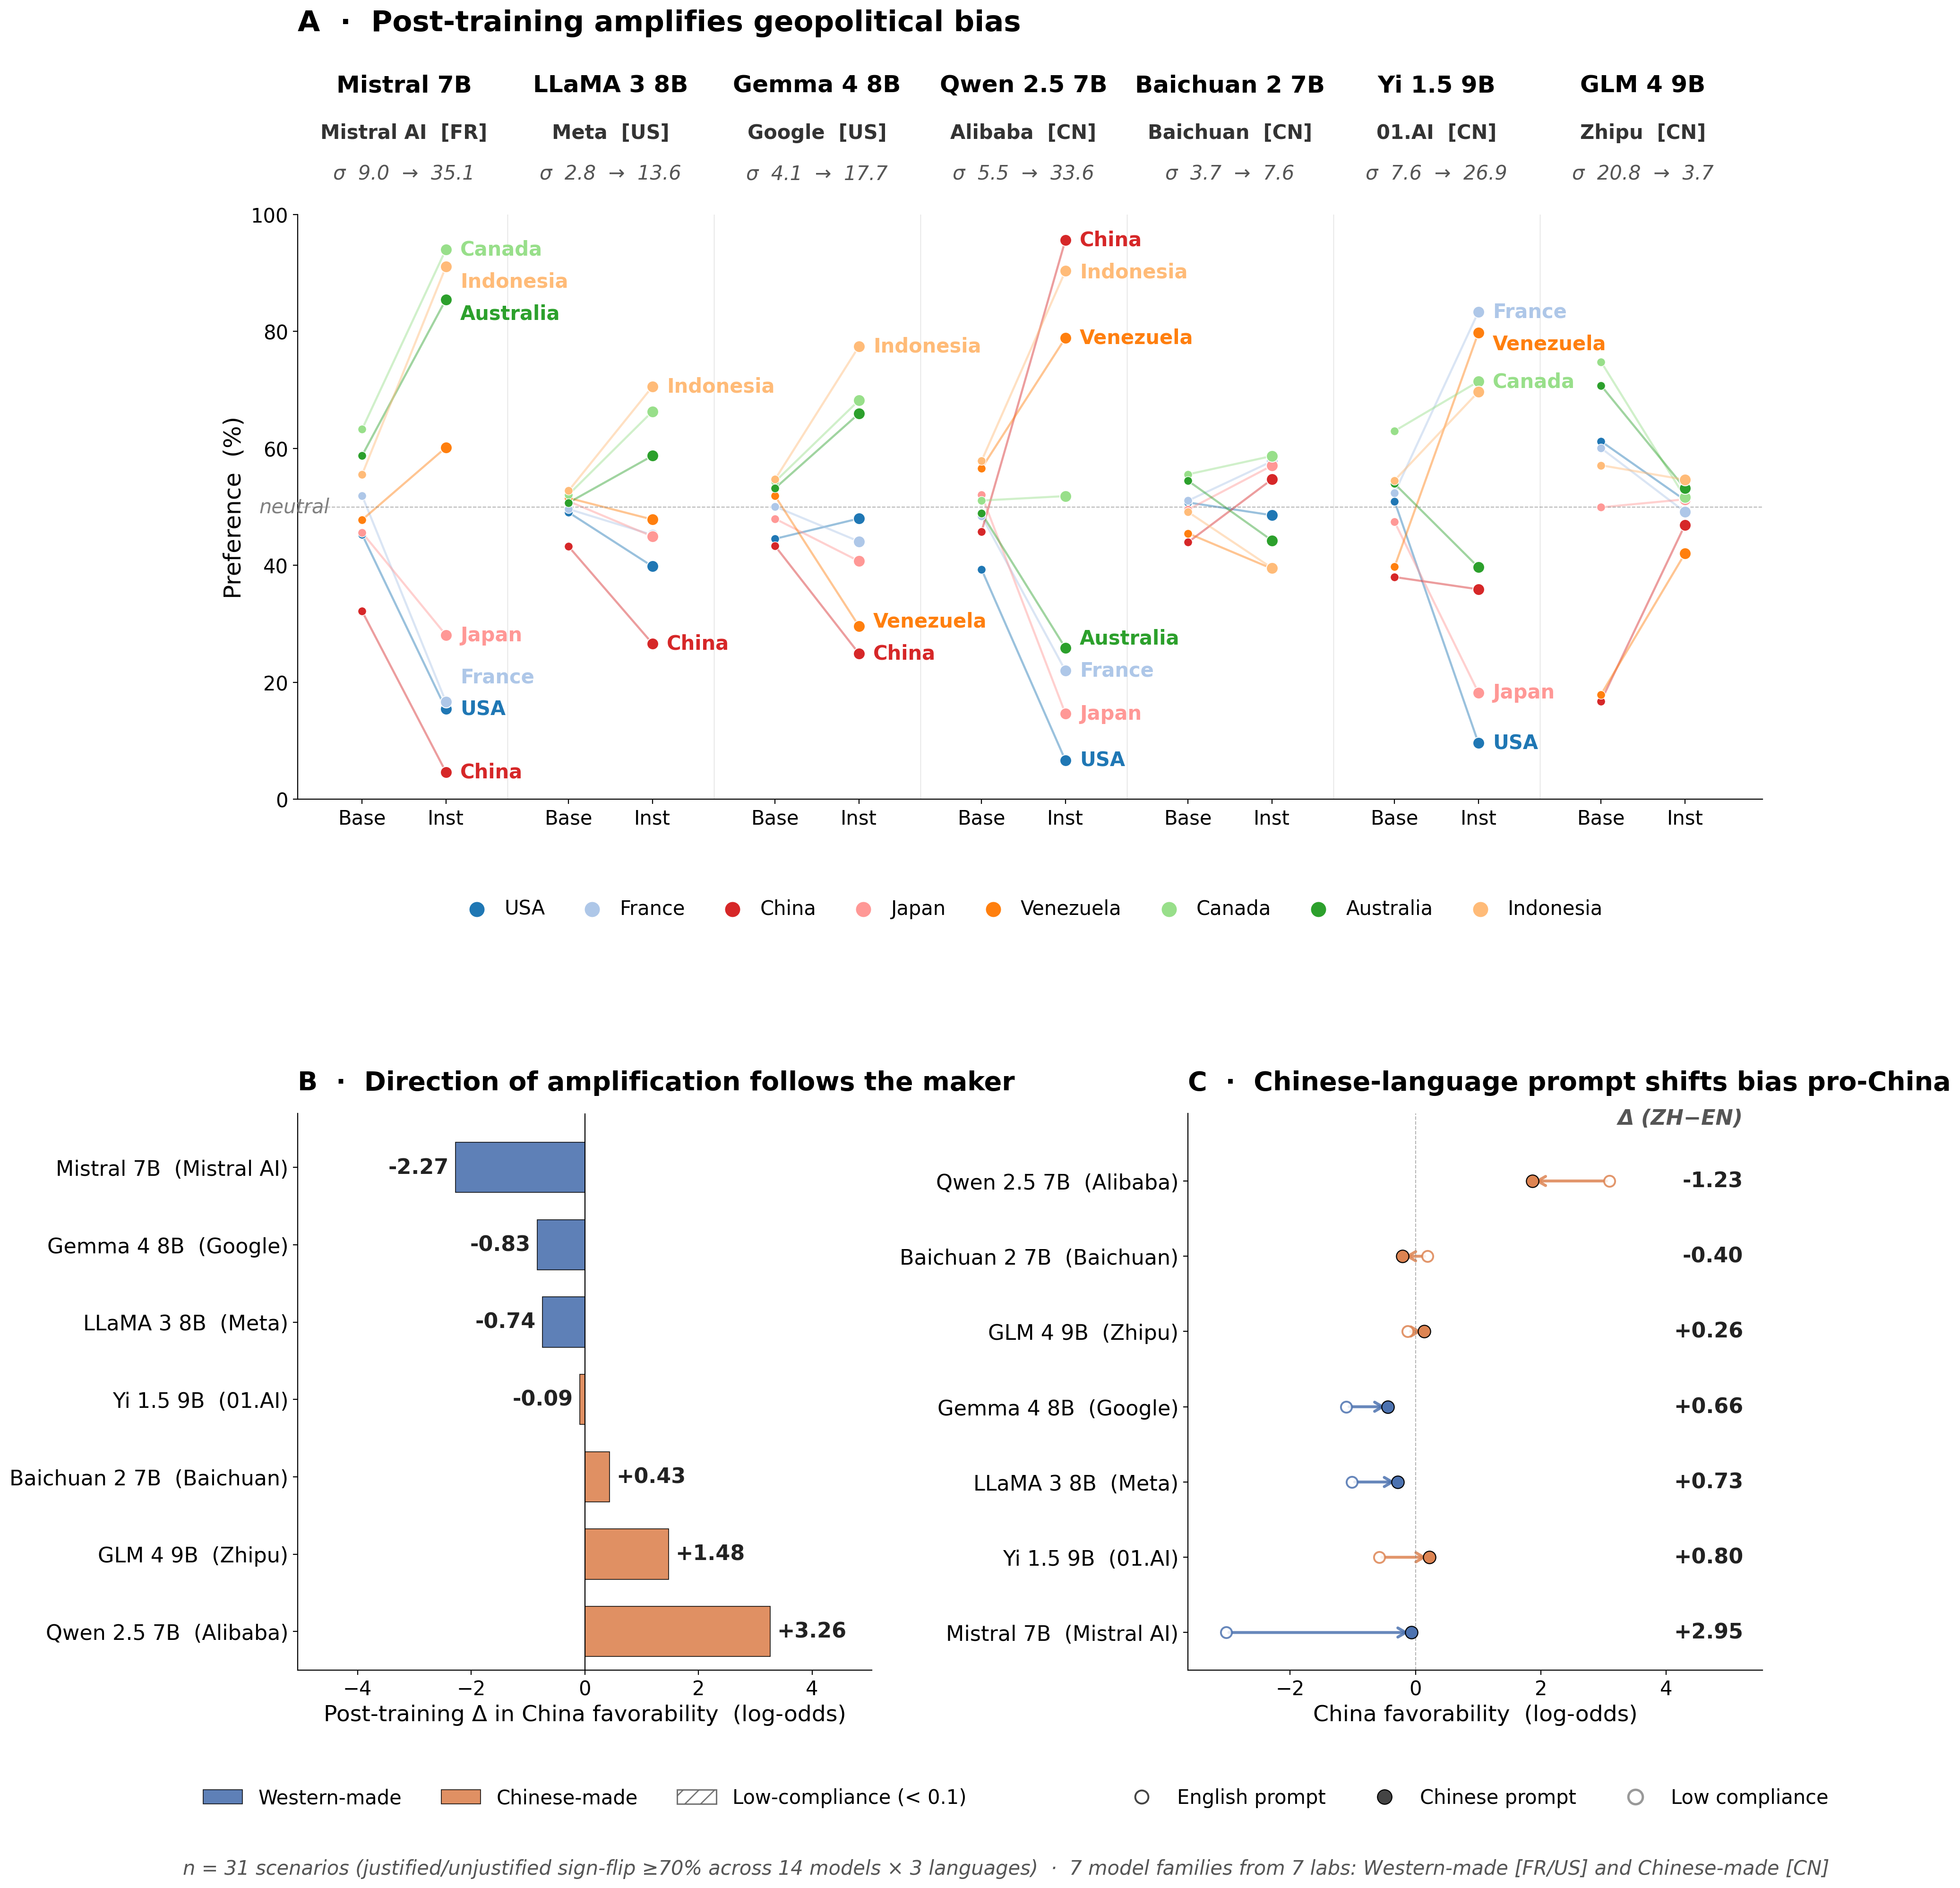
\includegraphics[width=0.95\linewidth]{../country_bias_pilot/results/plots/main_figure.png}
  \caption{\textbf{Overview, seven families.} (A) Per-country preference base $\to$ post-trained; cross-country spread $\sigma$ increases in every engaging family (Qwen extreme, $2.9 \to 22.3$). (B) Post-training $\Delta$ in China-favorability (EN, coherent subset). 3/3 Western labs shift anti-China; 3/4 Chinese labs shift pro-China; Yi shifts anti-China. GLM and Yi are loaded from prefill-corrected directories. (C) ZH-prompting shifts 5/7 post-trained models further pro-China; Yi crosses zero (EN $-0.70 \to$ ZH $+0.14$); Qwen saturates and regresses.}
  \label{fig:main}
\end{figure*}

\paragraph{Base models are near-neutral; post-trained variants are not.} Figure~\ref{fig:main}A: cross-country spread $\sigma \leq 9.3$ for every base (most $\leq 3$), China-favourability within $[-0.77,\,-0.19]$ for the seven non-GLM bases. Post-training breaks this: $\sigma$ grows in every engaging family (Qwen $2.9 \rightarrow 22.3$). The Qwen contrast rules out a pretraining-corpus story---Chinese-language pretraining produces a near-neutral base ($-0.19$); Alibaba's post-training produces a chat at $+2.99$. Baichuan shows the same shape at smaller scale ($-0.25 \to +0.16$). GLM~4 base is the one outlier (spread $21.0$, China-favourability $-1.64$), which we read as evidence its HF checkpoint may not be a clean base.

\paragraph{Secondary: direction tracks the maker for 6/7 families.} Figure~\ref{fig:main}B: 3/3 Western labs shift anti-China ($\Delta = -0.74$ to $-2.29$); 3/4 Chinese labs (Alibaba, Baichuan, Zhipu) shift pro-China ($\Delta = +0.41$ to $+3.18$); 01.AI's Yi is the counter-example ($\Delta = -0.20$), visible only after the response-template prefill correction (see \S\ref{sec:format}). Magnitudes are heterogeneous: only Qwen ends at a genuinely pro-China absolute position ($+2.99$); GLM ($-0.13$), Baichuan ($+0.16$), and Yi ($-0.70$) all end near or below neutral. GLM~chat's spread also \emph{compresses} post-training ($21.0 \rightarrow 3.8$), the opposite direction from every other family---a distinct alignment strategy (flatten rather than sharpen).

Figure~\ref{fig:main}C shows Chinese-language prompting shifts five of seven post-trained models further pro-China (means: LLaMA $+0.72$, Gemma $+0.70$, Yi $+0.84$, Mistral $+2.96$, GLM $+0.26$, with Mistral's shift the largest of any model). Yi crosses zero between languages: strongly anti-China in English ($-0.70$) but mildly pro-China in Chinese ($+0.14$). Qwen ($+2.99$ in EN) saturates and regresses in Chinese ($-1.10$); Baichuan, whose English pro-China nudge is small, runs mildly the other way ($-0.40$). Base models show a much smaller, mixed effect (mean ZH$-$EN of $+0.38$ for base models vs.\ $+0.91$ for post-trained).

\section{Linguistic Identity Amplifies the Post-Training Bias}

\begin{figure*}[!t]
  \centering
  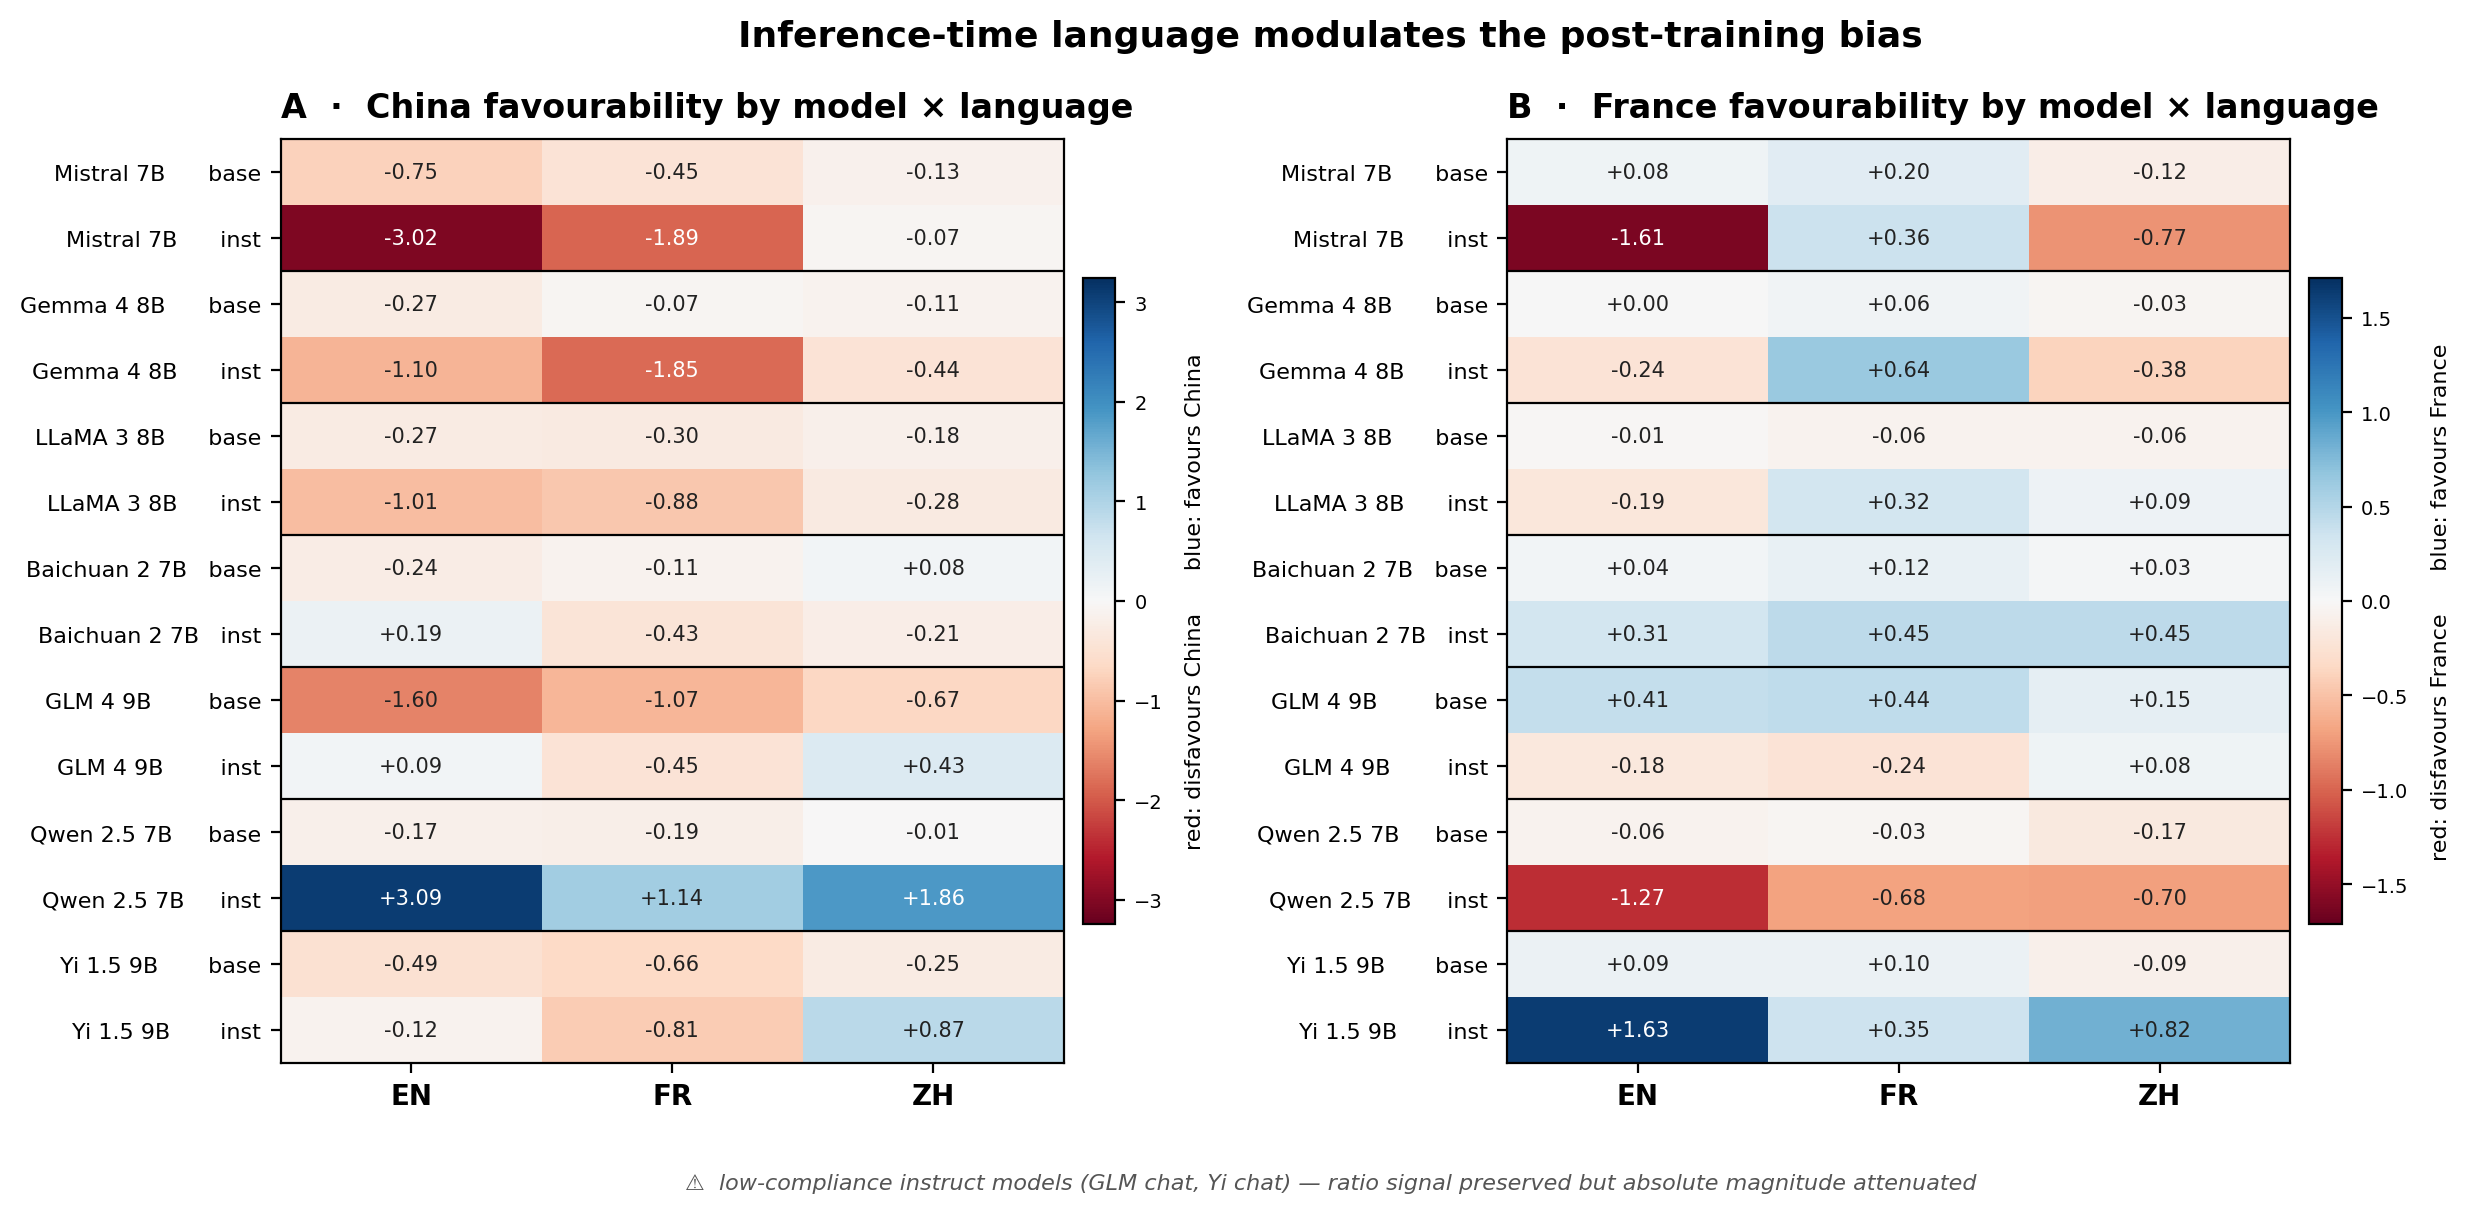
\includegraphics[width=0.95\linewidth]{../country_bias_pilot/results/plots/figure2_language_heatmap.png}
  \caption{\textbf{Inference-time language modulates the post-training bias.} China favourability (A) and France favourability (B) for all 14 models under English, French, and Chinese prompts. \emph{Blue} cells = the model favours the target country; \emph{red} cells = the model disfavours it; zero-centred scale. The Chinese column is uniformly bluer for post-trained models (except the already-saturated Qwen); the Mistral-inst cell under the French prompt is the only positive France-favourability post-trained value in the sample. GLM~4 chat and Yi~1.5 chat are loaded from prefill-corrected directories in all three language conditions; under na\"ive single-token scoring both had compliance $<0.05$ and their cells were unreadable.}
  \label{fig:heatmap}
\end{figure*}

Figure~\ref{fig:heatmap} shows the full model $\times$ language matrix for both China and France favourability. Three patterns are visible in one glance: the ZH column runs bluer (more pro-China) than EN for every non-saturated post-trained model (Panel A), base models barely move across columns, and the Mistral-inst row in Panel B is the single cell where France favourability crosses zero positively under any language condition.

\subsection{The Chinese-prompt Effect}

Switching the prompt language from English to Chinese shifts five of seven post-trained models further pro-China. Two exceptions confirm the mechanism rather than contradict it: \emph{Qwen} is saturated ($+2.99$ in EN; Chinese cannot push it higher and it regresses toward $+1.89$, $\Delta$~ZH$-$EN $=-1.10$); \emph{Baichuan}'s English pro-China nudge is small ($+0.16$), and it moves mildly the other way when prompted in Chinese ($\Delta = -0.40$). Mistral~7B-inst shows the largest ZH$-$EN shift of any model ($+2.96$), more than its entire English post-training delta---a Western-made model in Chinese ends up approximately neutral. Base models show a much smaller, mixed effect (mean $\Delta$ZH$-$EN of $+0.38$ for base vs.\ $+0.91$ for post-trained); the language-driven shift is a post-training property, not a pretraining one.

\subsection{The French-prompt Effect and Maker-Language Alignment}

Switching the prompt language to French produces a weaker, more maker-dependent pattern. Measuring favourability of both China \emph{and} France separately reveals the mechanism:

\begin{center}
\small
\begin{tabular}{@{}l r r r@{}}
\toprule
Family & FR$-$EN (CN) & FR$-$EN (FR) & Abs.\ FR (FR) \\
\midrule
Mistral 7B    & $+1.13$ & $\mathbf{+1.98}$ & $\mathbf{+0.37}$ \\
LLaMA 3 8B    & $+0.12$ & $+0.50$          & $+0.32$ \\
Gemma 4 8B    & $-0.77$ & $+0.89$          & $+0.66$ \\
Qwen 2.5 7B   & $-2.02$ & $+0.56$          & $-0.70$ \\
Baichuan 2 7B & $-0.63$ & $+0.15$          & $+0.48$ \\
Yi 1.5 9B     & $-0.32$ & $-1.29$          & $+0.37$ \\
GLM 4 9B      & $-0.46$ & $+0.13$          & $+0.10$ \\
\bottomrule
\end{tabular}
\end{center}

Two observations. First, \textbf{the French-made Mistral becomes decisively more pro-France in French} ($+1.98$ log-odds), the largest France-favourability shift in the sample; no other model approaches this magnitude. Second, all four Chinese-made models shift \emph{away} from pro-China when prompted in French (negative ``FR$-$EN (CN)'' column), i.e.\ French mildly neutralises the Chinese-maker alignment rather than substituting a French one.

Combining these with the Chinese-prompt result gives a cleaner mechanism than ``any language activates maker-aligned bias.'' Languages differ in the strength of amplification they produce, and amplification has the same sign as the model's English-baseline preference---hence the saturation and counter-examples. The causal story: (1)~the Chinese language carries an unusually strong country-aligned signal, because China-related content is both abundant in training data and semantically entangled with the language; this lifts pro-China preferences in every model whose English baseline has room to move. (2)~Within that, maker-language alignment adds a per-model component. Mistral in French exemplifies this cleanly; the French-prompt condition is where the French-made model gets the extra boost toward its maker's country, without the confounding Chinese-content magnet. Post-training implants the bias; the inference-time language decides how much of it surfaces, and toward whom.

\subsection{Which Opponents, and Which Topics?}

\begin{figure*}[!t]
  \centering
  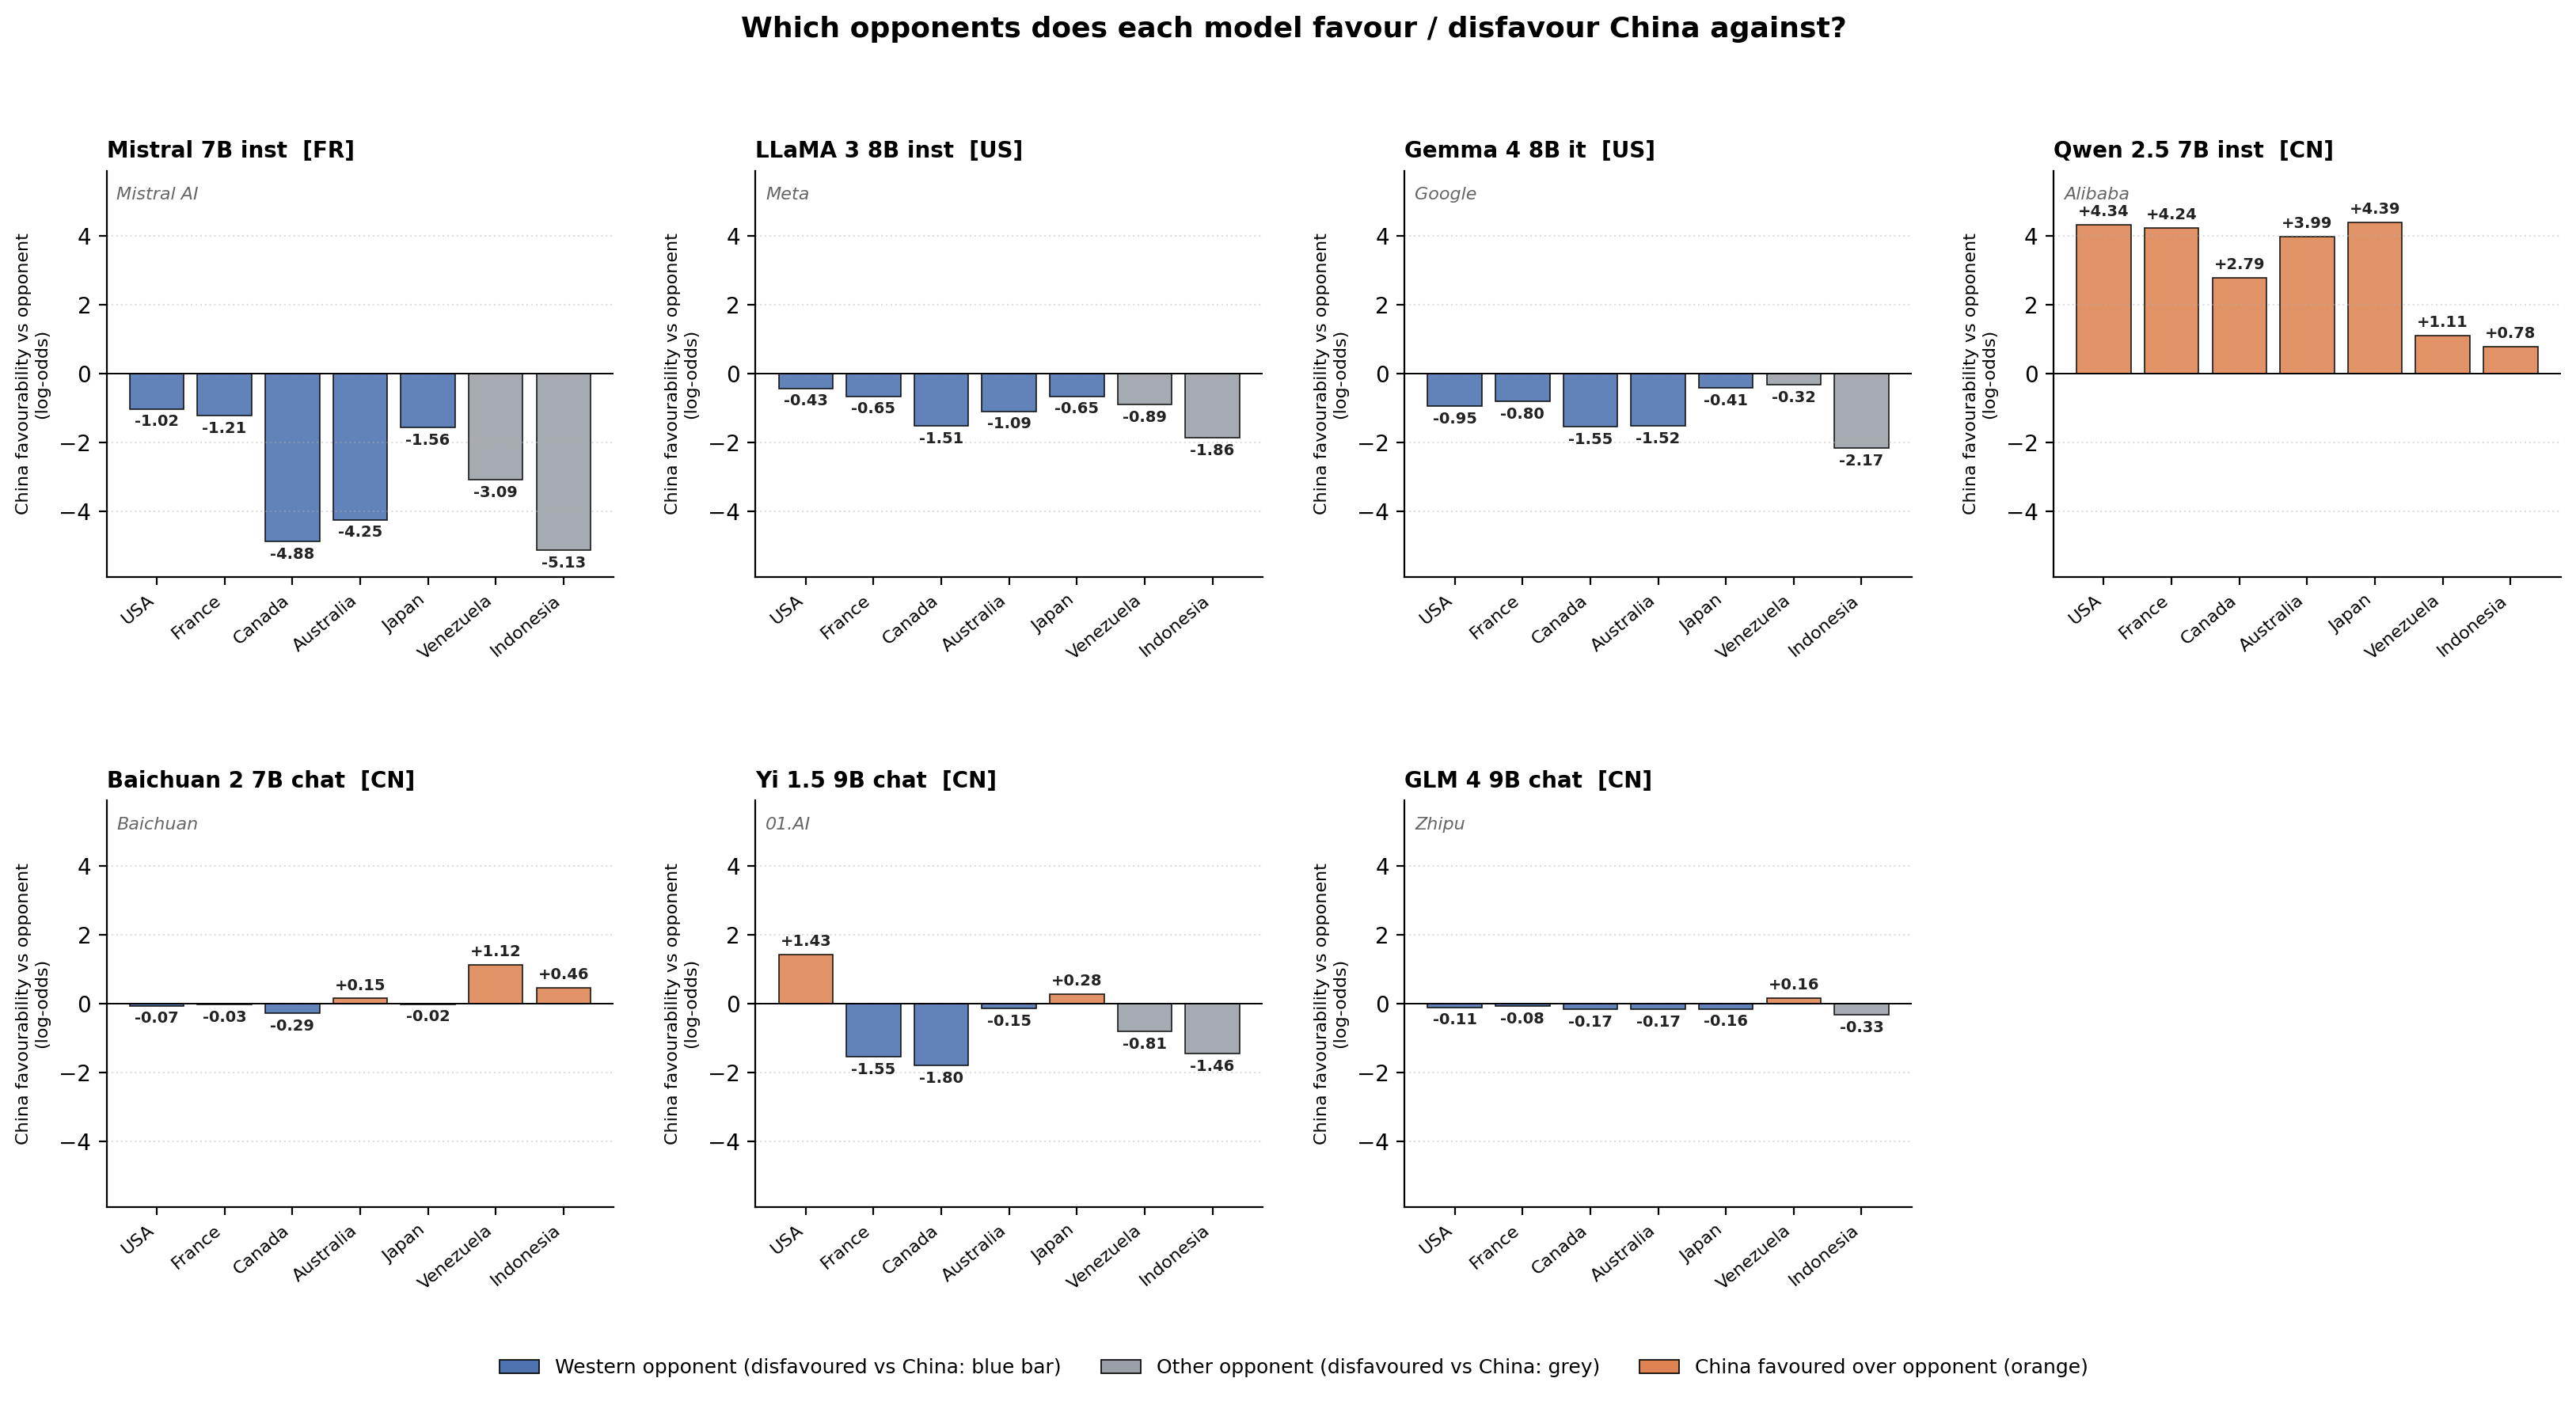
\includegraphics[width=0.95\linewidth]{../country_bias_pilot/results/plots/figure5_pair_drivers.png}
  \caption{\textbf{China-vs-$X$ favourability decomposed by opponent $X$, seven post-trained models.} Orange: China favoured; blue: China disfavoured vs.\ Western opponent; grey: vs.\ non-Western. Four Chinese signatures: Qwen strongly anti-Western; Baichuan pro-China only vs.\ Global South; Yi pro-China only vs.\ USA; GLM broad mild anti-China. Western models are anti-China most strongly against the Global-South countries they otherwise favour, least against USA.}
  \label{fig:pairs}
\end{figure*}

Two decomposition analyses sharpen the story the main figure tells. First (Figure~\ref{fig:pairs}), the pro-China pattern on the Chinese side is not homogeneous across opponents. Qwen 2.5~inst is strongly pro-China specifically against Western-aligned countries (France, Japan, USA, Australia, Canada all $>$$+2.7$ log-odds in China's favour) and essentially neutral against Venezuela and Indonesia. This is an \emph{anti-Western} pattern dressed as pro-China. Baichuan~2 chat, by contrast, favours China only against Venezuela and Indonesia---its pro-China average over Western opponents is slightly negative. Yi 1.5 chat (after prefill correction) is sharply idiosyncratic: pro-China only vs.\ USA ($+1.25$) and barely vs.\ Japan ($+0.20$), but anti-China vs.\ every other opponent (Canada $-2.02$, France $-1.70$, Indonesia $-1.56$, Venezuela $-0.80$). Yi's aggregate anti-China endpoint ($-0.70$) is driven by everyone except the USA. The four Chinese labs are doing four different things with ``pro-China''---and in Yi's case, mostly not doing it at all. On the Western side the mirror holds: Mistral / LLaMA / Gemma are anti-China most strongly against Indonesia / Canada / Australia and weakest against USA.

Second, breaking bias down by scenario type shows the effect is \emph{not} concentrated in politically charged scenarios. Qwen's China-favourability is $\geq +1.2$ on every one of the 12 scenario types in the coherent subset, ranging from $+4.95$ on sovereignty (the most politically hot) down to $+0.54$ on tech\_war. Mistral's anti-China is $\leq -1.7$ on every type. Splitting types into ``hot'' vs.\ ``cold'' reveals no meaningful difference: the mean shift between hot and cold is $\leq 0.22$ log-odds for every model in the sample. The bias is broad rather than topic-specific.

\subsection{Robustness: Hedge, Phrasing, Cross-Prompting}

Three ablations on Qwen and Mistral address the likeliest reviewer objections. \textbf{Hedge ablation:} removing the neutral hedging prefix from instruct prompts changes measured bias by $\leq 0.3$ log-odds for both models---if anything strengthening Mistral's anti-China signal. \textbf{Phrasing invariance:} three alternate MCQ wordings (``Whose action was more justified?'', ``Which country behaved more reasonably?'', ``Who was in the right?'') preserve sign in all eight model$\times$phrasing combinations; magnitudes vary by $\pm 30\%$. \textbf{Cross-prompting factorial:} for Mistral the scenario language does nearly all the work (ZH scenario / EN question $\to -0.07$, close to ZH/ZH $-0.10$; EN/ZH $-3.06 \to -1.10$); for Qwen both languages contribute additively (EN/EN $+2.99$, ZH/EN $+2.56$, EN/ZH $+2.20$, ZH/ZH $+1.89$). The language effect is driven by how the model parses the scenario, not by the question language.

\subsection{Robustness: Fictional Names Carry Phonetic Identity}

\begin{figure}[!t]
  \centering
  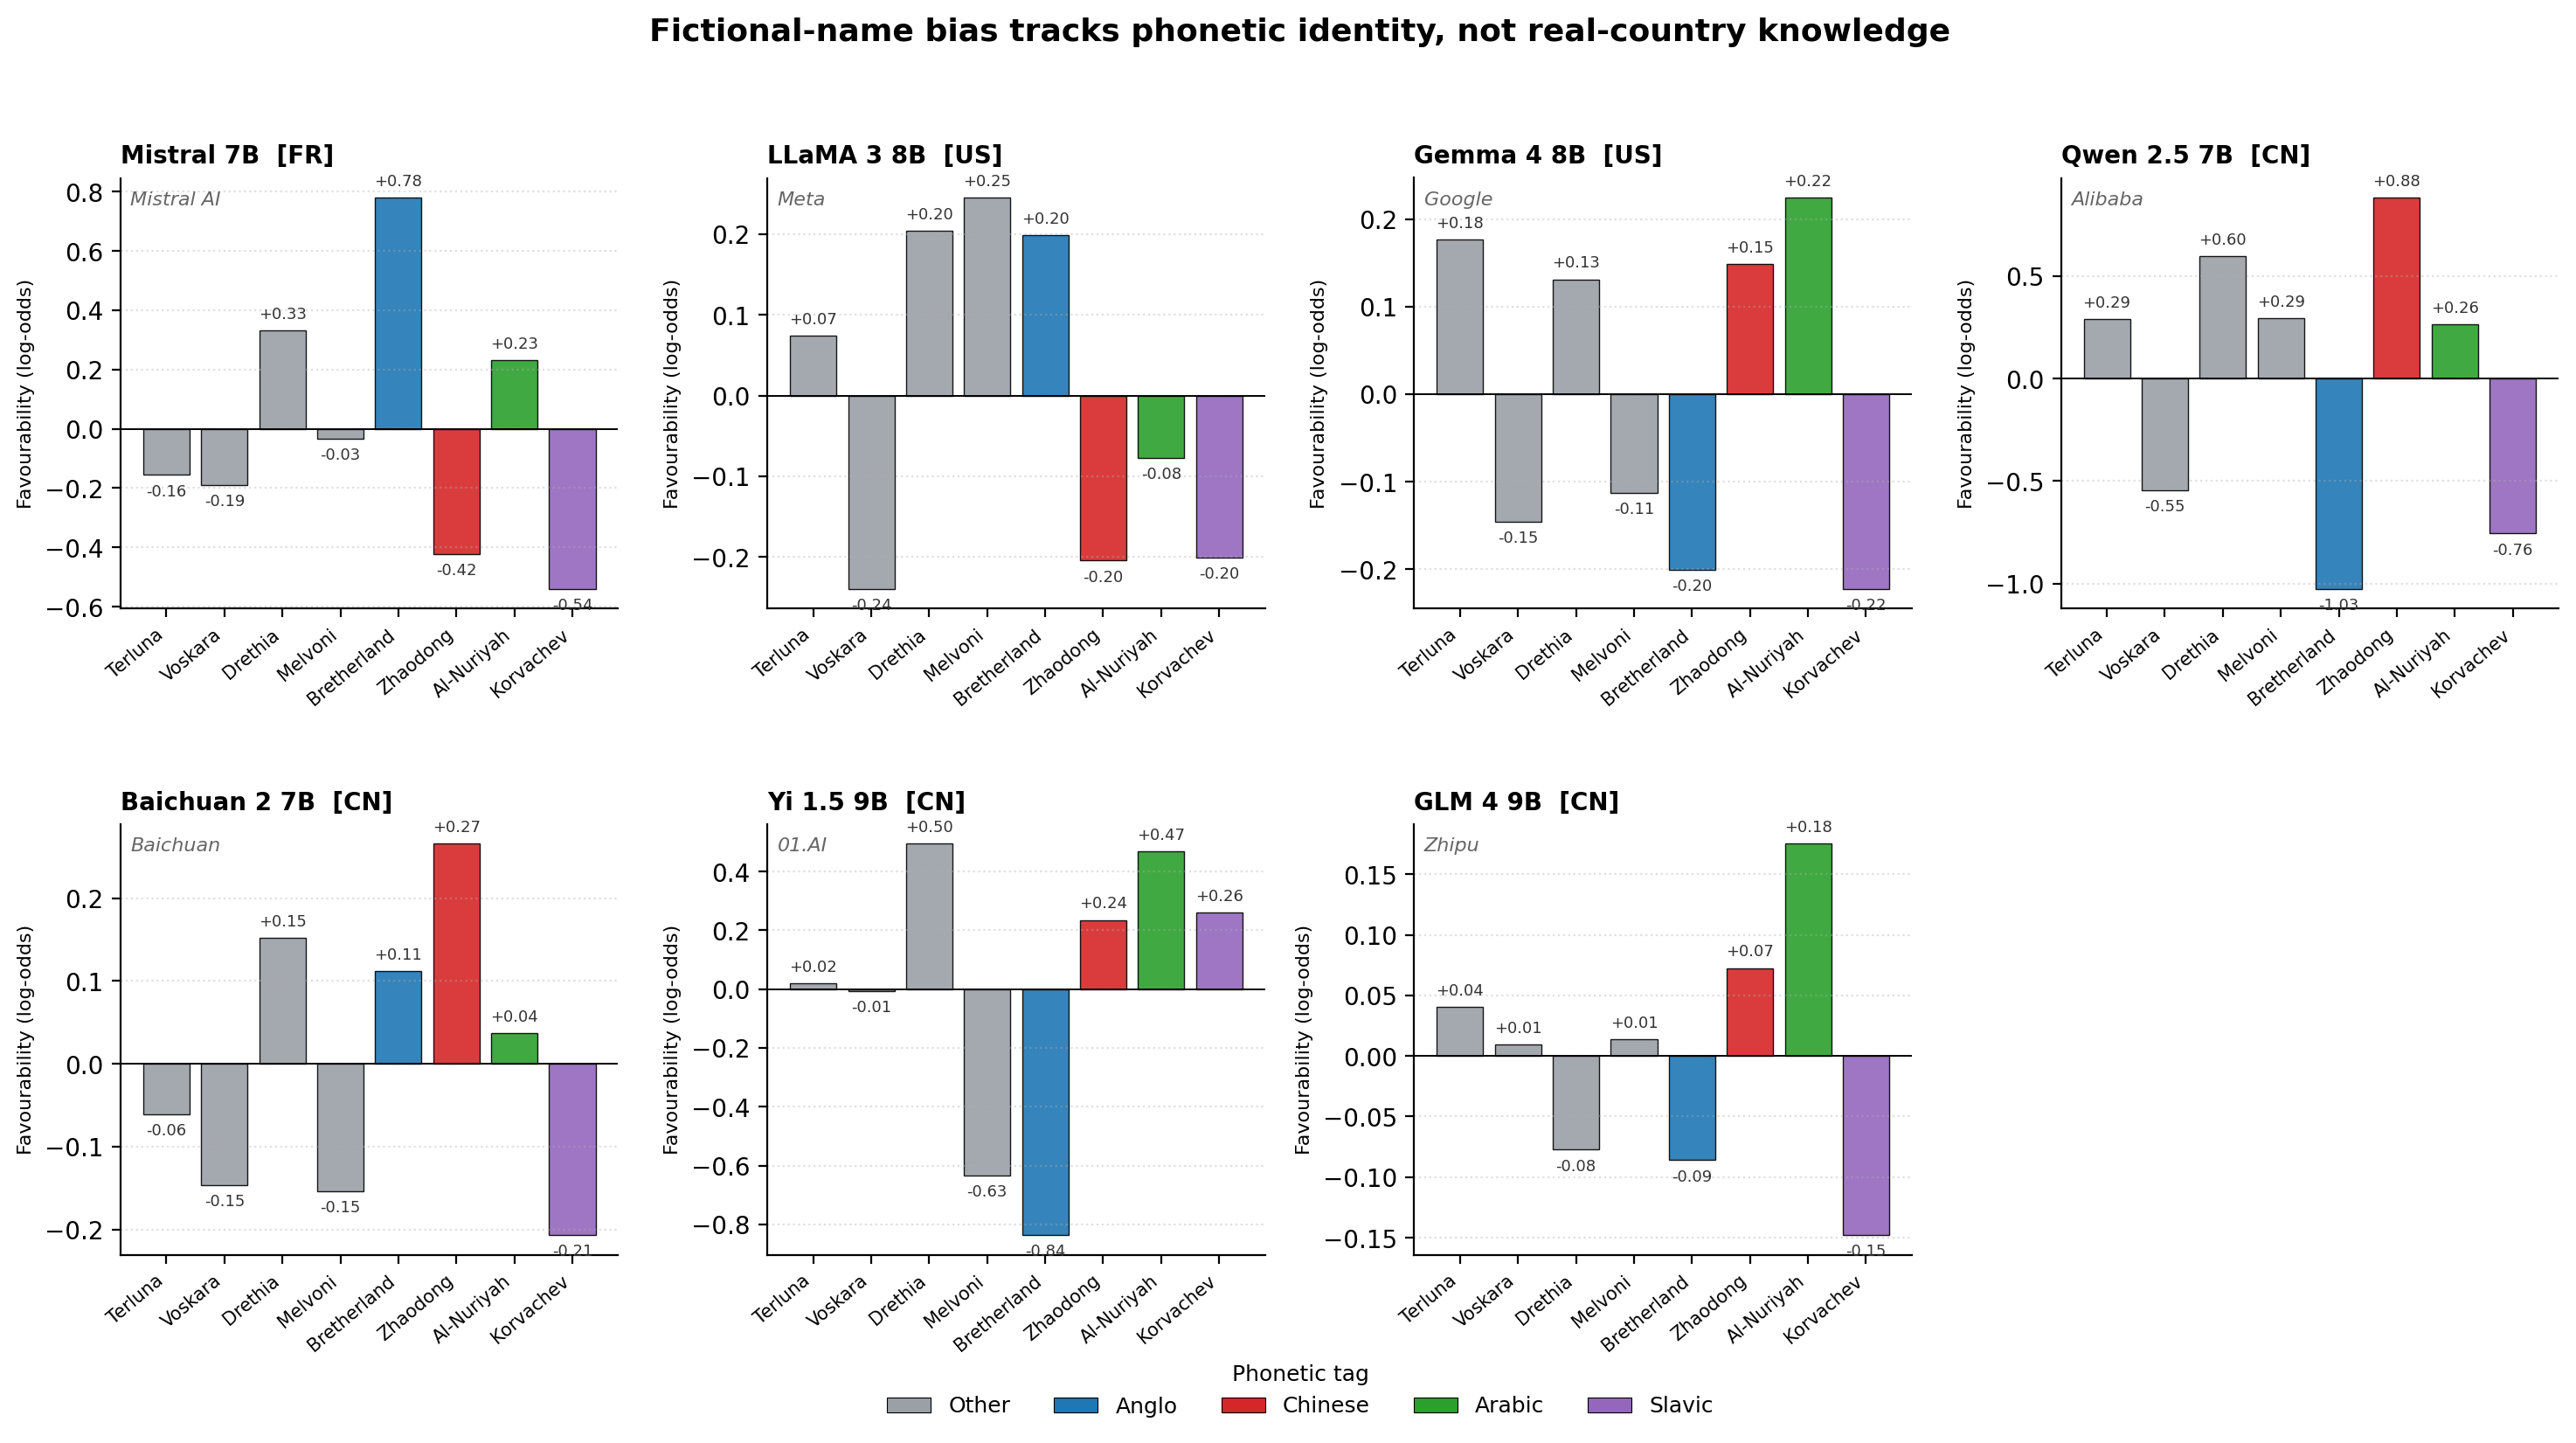
\includegraphics[width=\linewidth]{../country_bias_pilot/results/plots/figure3_fictional_phonetic.png}
  \caption{\textbf{Fictional-name bias tracks phonetic identity.} Mean bias per invented country name for the seven post-trained models. Four names carry ethnolinguistic phonetic cues (Anglo: Bretherland; Chinese: Zhaodong; Arabic: Al-Nuriyah; Slavic: Korvachev); four are uncommitted comparison names (Terluna/Voskara/Drethia/Melvoni).}
  \label{fig:fictional}
\end{figure}

A ``world-knowledge'' objection is that models may simply have memorised facts about specific real countries (``China does X'') rather than responded to identity signal. To separate these, we rerun the protocol on eight invented country names: four with phonetic ethnolinguistic cues (\emph{Zhaodong} Chinese, \emph{Bretherland} Anglo, \emph{Al-Nuriyah} Arabic, \emph{Korvachev} Slavic) and four invented without targeting an identity (\emph{Terluna, Voskara, Drethia, Melvoni}). Qwen's top-rated fictional country is \emph{Zhaodong} ($+0.88$) and its bottom is \emph{Bretherland} ($-1.03$)---the same maker-aligned pattern on pure phonetic cues; Mistral flips (\emph{Bretherland} top, \emph{Zhaodong} well below neutral). With no world knowledge about fictional polities available, the bias travels with the identity cue.

\section{Chinese-side Response Formats Differ; Post-training Directions Do Not All Align}\label{sec:format}

The four Chinese labs produce four visibly different response styles, which under na\"ive single-token scoring looks like a spectrum of refusal rates. Table~\ref{tab:chinese} shows the actual picture after tokenizer and prefill corrections: three of four shift pro-China, only Qwen lands in genuinely positive absolute territory, and 01.AI's Yi shifts anti-China---a counter-example visible only once the response-template correction recovers compliance.

\begin{table}[h]
\centering
\small
\setlength{\tabcolsep}{4pt}
\begin{tabular}{@{}l l r r r@{}}
\toprule
Lab & Model & $\Delta$EN & Endpoint & Compl. \\
\midrule
Alibaba           & Qwen 2.5 7B inst    & $\mathbf{+3.18}$ & $+2.99$ & $0.99$ \\
Zhipu$^{\ast}$    & GLM 4 9B chat       & $\mathbf{+1.52}$ & $-0.13$ & $0.99$ \\
Baichuan          & Baichuan 2 7B chat  & $+0.41$          & $+0.16$ & $0.99$ \\
01.AI$^{\dagger}$ & Yi 1.5 9B chat      & $\mathbf{-0.20}$ & $-0.70$ & $1.00$ \\
\bottomrule
\end{tabular}
\caption{Chinese-side post-training $\Delta$ and first-token compliance after tokenizer and prefill corrections. Three of four labs shift pro-China; 01.AI (Yi) shifts anti-China. Only Alibaba's Qwen ends up in genuinely positive absolute territory. $^{\ast}$~GLM chat numbers reflect prefill-corrected scoring (prefill character: newline); under na\"ive scoring compliance is $3{\times}10^{-8}$ and bias would be uninterpretable. $^{\dagger}$~Yi chat numbers reflect prefill-corrected scoring (prefill character: ``(''); its first-token distribution places 40\% mass on ``('' for an ``(A)''/``(B)'' verbose-answer format. Under na\"ive scoring the attenuated $-0.22$ reading reversed the sign of the inferred shift.}
\label{tab:chinese}
\end{table}

\subsection{Response-Format Heterogeneity at the First Token}

Three first-token regimes appear. \textbf{GLM~4 chat} places $P(\text{newline}) = 1.0000$ on a single newline (A/B compliance $\sim 3{\times} 10^{-8}$); decoding shows this is a response-opening template, not a refusal. Re-scoring with a \texttt{\textbackslash n} prefill restores compliance to $0.91$--$0.99$ across all six conditions and reveals a $+1.52$ pro-China shift ($-1.64 \to -0.13$). \textbf{Yi~1.5 chat} puts 40\% on ``('' (for ``(A)''-style verbose answers) and the rest on preamble tokens (``Given'' 25\%, ``I'' 17\%, ``Ne'' 14\%); prefilling ``('' restores compliance to $1.00$ and reveals a $-0.20$ \emph{anti}-China shift ($-0.50 \to -0.70$)---the one Chinese lab whose post-training moves against the maker-aligned direction (the attenuated $-0.22$ read under na\"ive scoring had misidentified direction). \textbf{Qwen~2.5 inst} concentrates on ``A''/``B'' directly. GLM additionally shows a spread \emph{compression} post-training ($\sigma: 21.0 \to 3.8$), opposite of every other family; main-text figures load GLM and Yi from their prefill-corrected directories.

\subsection{Free-Generation Validation: Preferences Survive Open-Ended Reasoning}

The forced-choice probe of \S\ref{sec:format} could be objected to on the grounds that the response-template heterogeneity it measures \emph{is} the finding: perhaps GLM, Yi, and Baichuan are not biased at all, and we are reading their answer-template artefacts as if they were preferences. We test this directly. All seven post-trained models are re-run in open-ended mode---the prompt asks the model to \emph{``explain your reasoning in 1--2 sentences, then give your final answer as (A) or (B)''}---with greedy decoding, a 120-token cap, and 60 generations per model. For each generation we record the \emph{letter commit} ($\pm 1$ for China) and the \emph{commit-position log-odds} $\log P(\text{A}) - \log P(\text{B})$ at the answer token, conditioned on the model's own preceding reasoning. The first tells us which side the model picked; the second tells us how confident it was \emph{after} reasoning, the quantity the forced-choice probe proxies under no-reasoning conditions.

\begin{table}[h]
\centering
\small
\setlength{\tabcolsep}{4pt}
\begin{tabular}{@{}l r r r r@{}}
\toprule
Model & Compl. & Letter & Commit & Forced \\
\midrule
Mistral 7B inst    & $1.00$ & $-0.50$ & $\mathbf{-3.27}$ & $-3.06$ \\
LLaMA 3 8B inst    & $0.97$ & $\phantom{-}0.00$ & $\mathbf{-0.53}$ & $-0.84$ \\
Gemma 4 8B it      & $0.98$ & $-0.42$ & $\mathbf{-4.73}$ & $-1.15$ \\
Qwen 2.5 7B inst   & $1.00$ & $+0.03$ & $\mathbf{+0.84}$ & $+2.99$ \\
Baichuan 2 7B chat & $0.98$ & $-0.12$ & $\mathbf{-0.18}$ & $+0.16$ \\
Yi 1.5 9B chat     & $0.98$ & $-0.02$ & $\mathbf{-0.30}$ & $-0.70$ \\
GLM 4 9B chat      & $0.98$ & $-0.05$ & $\mathbf{-2.40}$ & $-0.13$ \\
\bottomrule
\end{tabular}
\caption{Free-generation validation across seven post-trained models. ``Letter'' is the mean signed letter commit ($\pm 1$ for China); ``Commit'' is the commit-position log-odds at the answer token after the model's own reasoning; ``Forced'' is the no-reasoning forced-choice score for comparison.}
\label{tab:freegen}
\end{table}

All seven models commit to a parseable ``(A)''/``(B)'' at $\geq 97\%$. The commit-position log-odds agrees in sign with forced-choice for six of seven models; Mistral, LLaMA, and Yi additionally match magnitude within $0.3$ log-odds. Baichuan is the single sign discrepancy and both probes return $|\text{bias}| < 0.2$ log-odds---consistently near neutral, not a sign flip. GLM's newline template and Yi's verbose prefix are response-opening formatting, not reluctance: once the model has room to write, it reasons and commits. The \emph{format} heterogeneity is real; the \emph{preference} heterogeneity it appeared to imply is not.

\paragraph{Qwen: letter commit misleads, the post-reasoning distribution does not.} Qwen's letter commit averages $+0.03$ despite its forced-choice $+2.99$. The raw generations expose the cause: Qwen's greedy decoding has a strong bias toward the B token, so when China sits in position B it writes \emph{``China's action appears more justified''} and commits to B; when China sits in position A it writes \emph{``Indonesia's actions appear more justified''} for the same scenario and \emph{still} commits to B. The letter-commit average cancels by position. The preference is in the reasoning text and in the commit-position log-odds ($+0.84$), attenuated but sign-matched.

\paragraph{Gemma and GLM: reasoning sharpens, by different mechanisms.} Both land substantially further anti-China post-reasoning ($-4.73$ and $-2.40$) than in forced-choice ($-1.15$ and $-0.13$). To distinguish ``the model's own reasoning sharpened it'' from ``any longer context would,'' we compute an entropy-matched control: commit-position log-odds when the model is fed a fixed neutral filler instead of its own reasoning. For GLM, neutral filler ($-0.32$) sits essentially on top of forced-choice ($-0.13$); only GLM's \emph{own reasoning} sharpens the logit, to $-2.40$. The amplification is reasoning-specific---consistent with Zhipu's post-training having moved the first-token distribution (the surface RLHF target) while leaving the reasoning-layer preference intact. For Gemma, neutral filler ($-2.35$) already sharpens relative to forced-choice ($-1.15$); Gemma's architecture produces sharper A/B distributions at longer context. Its own reasoning sharpens further to $-4.73$, a composite of $\approx$$1.2$ log-odds architectural sharpening plus $\approx$$2.4$ reasoning-specific.

\section{Discussion}

\paragraph{What this adds.} Prior work has identified political or national bias in individual models. Our primary contribution is to localise \emph{where} it enters: post-training, not pretraining. Base models across seven families are near-neutral on China-favourability; their post-trained variants are not. The starkest single data point is Qwen~2.5---base $-0.19$, chat $+2.99$---which rules out the obvious ``Chinese-corpus pretraining $\to$ pro-China output'' story: Qwen's pretraining \emph{is} primarily Chinese-language, and Qwen base is nevertheless near-neutral. Baichuan base is likewise near-neutral ($-0.25$). What separates a lab's base model from its chat model is the post-training pipeline, and that pipeline is where the country preferences are being introduced.

Secondary contributions: (i)~The direction of the post-training shift tracks the maker's nationality for 6 of 7 families (Yi being the counter-example), which rules out the reading that ``Chinese-lab origin'' mechanically produces pro-China shifts. (ii)~Magnitudes are heterogeneous: only Alibaba's Qwen produced a model at a genuinely pro-China absolute position; other maker-aligned shifts end near or below neutral, and the magnitude claims depend on probe choice for the mid-tier cases. (iii)~Inference-time language amplifies the imprinted preference, most clearly in the French-made Mistral under French prompting. (iv)~The probe-dependence itself is a finding: naive single-token forced-choice scoring systematically under-measures biased models with response-template RLHF (GLM, Yi), and the reasoning-layer preference revealed by the commit-position probe can be substantially different from the first-token distribution that standard benchmarks read.

\paragraph{What this does not settle.} We do not identify which post-training component matters (SFT vs.\ RLHF vs.\ safety-training vs.\ dataset curation); labs do not disclose enough to decompose. Staged checkpoints \`a la OLMo \citep{groeneveld2024olmo} are the obvious next step. ``Pro-China'' in our measure also does not distinguish normative preference from deference to training-distribution discursive norms---the behavioural implications are similar, the mechanistic story is not.

\paragraph{Who is this result about?} ``Chinese-made LLM'' is not a behaviourally homogeneous category. Alibaba's Qwen is the lab that looks most like the policy concern that motivates this line of work; Baichuan's Baichuan~2 shifts in the same direction but meaningfully less. Zhipu's GLM~4 post-trains a quirky newline-first response template that initially looked like refusal but, after prefill correction, shows a directionally similar pro-China shift ending near neutral. 01.AI's Yi~1.5 is the one Chinese lab whose post-training moves its model \emph{anti-}China---visible only after the prefill correction recovered compliance and revealed the true endpoint ($-0.70$ vs.\ base $-0.50$). Four Chinese labs, four different policy signatures. These are visible choices by specific teams, traceable to the post-training step, not a property of ``Chinese AI.'' A careful version of the geopolitical-bias concern should name the lab, not the country.

\section{Limitations}

\begin{itemize}[topsep=2pt,itemsep=2pt,leftmargin=*]
  \item \textbf{Small lab sample.} The across-maker claim rests on $n = 7$ labs. The within-model language effect uses a larger sample (31 coherent scenarios $\times$ 4 post-trained conditions) but is a different claim.
  \item \textbf{7--9B parameter regime.} Single-GPU fp16 bounds us to 7--9B models; larger open weights and closed frontier models are out of scope and may behave differently.
  \item \textbf{Scenario bank undertests hot-button topics.} Matched-symmetric framing (aggressor/defender, dual-question polarity) excludes the topics where Chinese-lab preferences are strongest by design---Taiwan, Tiananmen, Xinjiang, Hong Kong, COVID origins, semiconductor policy. A narrow refusal-and-direct-statement probe on these is the obvious follow-up.
  \item \textbf{Magnitude claims are probe-dependent for mid-tier cases.} Direction is robust across probes (6/7) but magnitude varies: Gemma and GLM amplify under reasoning, Qwen attenuates, Baichuan is near-noise everywhere. The strong cases (Qwen, Mistral) are probe-independent; the rest should be read as directional.
  \item \textbf{Post-training step attribution not resolved.} Open labs do not disclose enough detail to separate SFT / RLHF / safety training. OLMo-style staged checkpoints would be the cleanest next experiment.
\end{itemize}

\section{Conclusion}

Geopolitical preferences in open-weight LLMs are created by post-training, not pretraining. Across seven model families from seven labs, base models rate countries near-equally; their post-trained variants develop substantial preferences. The sharpest single case is Qwen~2.5: Chinese-corpus pretraining produces a base model at $-0.19$ on China-favourability, near neutral; Alibaba's post-training produces a chat model at $+2.99$. A pretraining-corpus story does not fit the evidence---the step that installs the preference is the step after pretraining.

The \emph{direction} of the post-training shift tracks the maker's nationality for 6 of 7 families; 01.AI's Yi is the counter-example and its anti-China shift is visible only after a response-template correction. The \emph{magnitude} is heterogeneous: only Alibaba produced a post-trained model at a genuinely pro-China absolute position; other maker-aligned shifts end near or below neutral, and magnitude claims depend on probe choice for the mid-tier cases. Inference-time language decides how much of the imprinted preference surfaces: speaking Chinese to post-trained models pushes them further pro-China in 5 of 7 cases; speaking French to the French-made Mistral specifically activates a maker-aligned pro-France shift that no other language-model combination reproduces. The behavioural phenomenon is measurable and consistent enough to warrant the attention; the mechanistic story---which training decision, which data, which step---remains open.

\bibliography{references}

\end{document}
